\section{Bayesian Model Averaging}
Suppose data $D$ could correspond to different models $M_k$, $k = 1, \dots, K$, and $\Delta$ is a quantity of interest. We have the posterior distribution:
\begin{equation}
p(\Delta|D) = \sum_{k=1}^K p(\Delta|M_k)\cdot p(M_k|D)
\label{eq:prior_Delta}
\end{equation}
where :
\begin{equation}
p(M_k|D) = \frac{p(D|M_k)\cdot p(M_k)}{\sum_{i=1}^Kp(D|M_i)\cdot p(M_i)}
\end{equation}
and :
\begin{equation}
p(D|M_k) = \int \underbrace{(D|\theta_k,M_k)}_{\text{likelihood}} \cdot p(\theta_k|M_k)d\theta_k
\end{equation}
\newline
In our case, we consider the solution given by the algorithm CAVI $q(z)$, which is a local optimum. To reach the global optimum, we will start the algorithm with different parameters. That way, we will obtain different optima and hopwefully, reach the global optimum. Then, we do a weighted average to find a plausible distribution.

\begin{figure}[h]
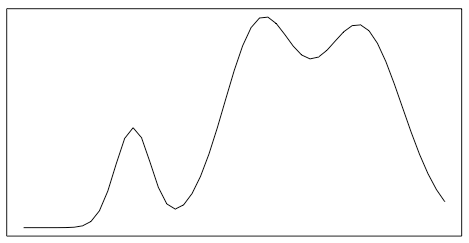
\includegraphics[width=4in]{images/localOptimum.png}
\caption{\label{fig:localOptimum}Depending on the starting parameters for \textit{CAVI} algorithm, it is possible to reach a local optimum that is not global. When using different starting points, the global optimum is reachable.}
\end{figure}